\chapter{Company Overview and General Project Framework}

\section{Introduction}
In an ever-evolving industrial context, companies are constantly seeking to enhance their performance through automation, robotics, and technological innovation. My final year project aligns with this trend and was carried out at Xpert-Meca, a company specialized in robot integration and the design and manufacturing of special-purpose machines.

This first chapter aims to present the overall context of the project, starting with a description of the host company, its activities, clients, and partners. It then transitions to a general presentation of the project, including its objectives and high-level operating principles, providing a solid foundation for the detailed technical information presented in subsequent chapters.

\section{Company Presentation}
\subsection{Introduction}
Founded in 2014 by a team of engineers experienced in mechanics, automation, and robotics, Xpert-Meca is an official partner of KUKA Robots. The company specializes in the integration and servicing of KUKA robots in Tunisia and North Africa, the design and production of special-purpose machines using numerical simulation, as well as industrial maintenance. Situated at Street Khaznadar in Hammam-Sousse, Sousse, Tunisia, the company's strategic placement facilitates access to key industrial networks and a skilled local workforce. Xpert-Meca provides complete and customized technical solutions for robots used in handling, welding, cutting, laser processing, polishing, packaging, and palletizing\hyperref[sec:bibliography]{[1]}.

The company adapts to its clients' products and production processes to design and deliver turnkey robotic solutions. The grippers, bases, conveyors, and all surrounding mechanical equipment are fully designed and manufactured by its in-house design office. The logos of Xpert-Meca and its official partner, KUKA, are shown in Figure \ref{fig:XPERT-MECA}.

\begin{figure}[H]
\centering

\includegraphics[width=0.6\textwidth]{Images/Chap1/KukaNxpert.png}
\caption[XPERT-MECA Logo and KUKA Logo]{XPERT-MECA Logo and KUKA Logo }
\label{fig:XPERT-MECA}
\end{figure}

\section{Xpert-Meca's Core Teams and Operations}
\subsection{Mechanical and Automation Development Team}

The mechanical development team includes experienced engineers and technicians responsible for designing and modeling mechanical components. Their expertise enables the creation of robust, precise, and reliable machines tailored to client needs. The automation team designs and programs control systems for the solutions. These professionals master the latest technologies and programming languages, ensuring smooth machine and process operation. A photo of the development teams is shown in Figure \ref{fig:XPERT-MECA_DevTeam}.

\begin{figure}[H]
\centering
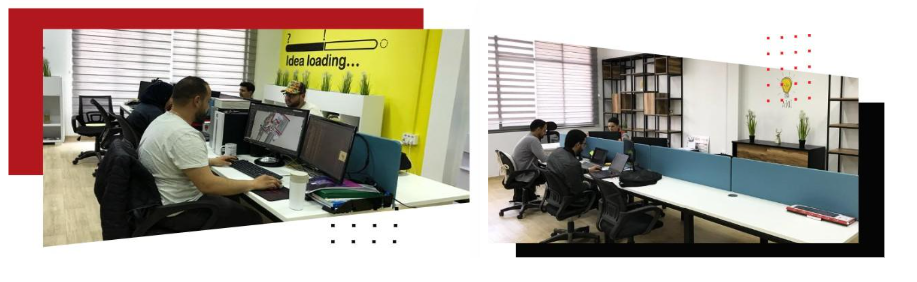
\includegraphics[width=1\textwidth]{Images/Chap1/DevTeam.png}
\caption[Mechanical Dev. Team and Automation Dev. Team]{Mechanical Dev. Team and Automation Dev. Team }
\label{fig:XPERT-MECA_DevTeam}
\end{figure}

\subsection{Robotics Team}
This team specializes in the integration and programming of industrial robots, which are central to Xpert-Meca’s core business. They are responsible for a full range of tasks, from the initial setup and calibration of robotic arms to the development of complex motion programs for diverse applications such as welding, handling, and palletizing. By working closely with clients, they develop custom robotic solutions that are meticulously designed to optimize production efficiency, ensure high precision, and enhance overall productivity. The team's expertise is critical to translating a client’s needs into a fully functional, automated robotic process, as shown in Figure \ref{fig:XPERT-MECA_Robotics}.

\begin{figure}[H]
\centering
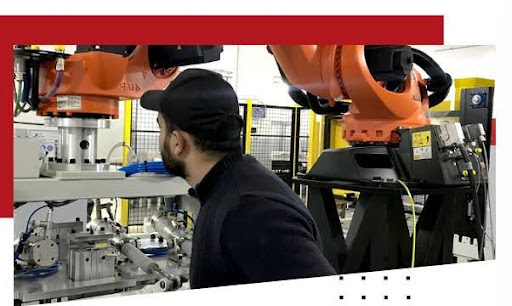
\includegraphics[width=0.6\textwidth]{Images/Chap1/RoboticTeam.jpg}
\caption[ Robotics team area]{ Robotics team area}
\label{fig:XPERT-MECA_Robotics}
\end{figure}

\subsection{Assembly Team}
The assembly team is responsible for the crucial final stage of system construction. They ensure that all designed and manufactured components—including mechanical structures, electrical panels, and pneumatic systems—are precisely and correctly assembled. Their work involves the meticulous installation and wiring of machines and systems according to detailed engineering plans. This team plays a vital role in verifying the physical integrity of the final product and ensuring that the mechanical and electrical installations are robust and perform optimally before the system is commissioned. The assembly zone is shown in Figure \ref{fig:XPERT-MECA_Assembly}.

\begin{figure}[H]
\centering
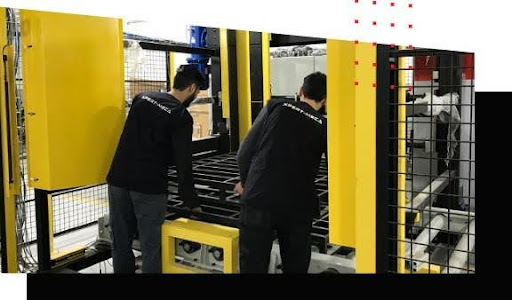
\includegraphics[width=0.6\textwidth]{Images/Chap1/AssemblyTeam.jpg}
\caption[ Assembly zone]{ Assembly zone}
\label{fig:XPERT-MECA_Assembly}
\end{figure}

\subsection{Machining Team}
This team is composed of skilled technicians who are experts in the production of high-precision mechanical parts. They operate a variety of advanced machinery, including CNC (Computer Numerical Control) machines, lathes, and milling machines, to fabricate custom components. The team’s work is essential for producing the specialized parts required for grippers, fixtures, and other bespoke equipment. Their expertise ensures that every component meets stringent quality and dimensional standards, which is fundamental to the reliability and performance of Xpert-Meca’s final products. The machining area is shown in Figure \ref{fig:XPERT-MECA_Machining}.

\begin{figure}[H]
\centering
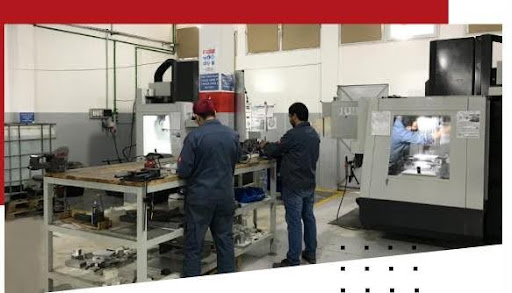
\includegraphics[width=0.6\textwidth]{Images/Chap1/MachiningTeam.jpg}
\caption[ Machining area]{Machining area}
\label{fig:XPERT-MECA_Machining}
\end{figure}

\subsection{Sales Team}
The sales team is the primary interface between Xpert-Meca and its clients. Their main focus is on customer satisfaction, providing support from the initial consultation through to the final purchase. The team is responsible for understanding client needs, offering tailored technical and commercial advice, and presenting solutions that align with the client’s operational and financial goals. They play a key role in building and maintaining strong customer relationships, which is vital for the company’s growth and market presence. The commercial area is shown in Figure \ref{fig:XPERT-MECA_Sales}.

\begin{figure}[H]
\centering
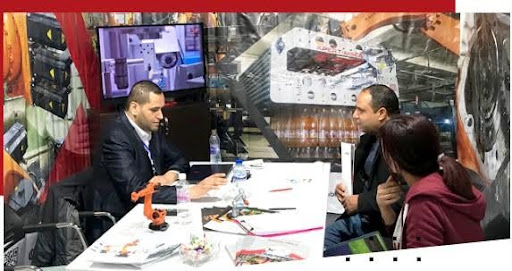
\includegraphics[width=0.6\textwidth]{Images/Chap1/Sales.jpg}
\caption[ Commercial area]{Commercial area}
\label{fig:XPERT-MECA_Sales}

\end{figure}

\subsection{After-Sales Service (SAV) Team}
Dedicated to ensuring the long-term operational continuity of installed systems, the After-Sales Service (SAV) team provides technical support and maintenance. Their role is to respond to client requests, troubleshoot issues, and perform routine maintenance to prevent system failures. This team’s effective and rapid response ensures that any downtime is minimized and that the installed solutions continue to operate reliably. Their work is crucial for upholding the company's reputation for quality and support. The after-sales service zone is shown in Figure \ref{fig:XPERT-MECA_AfterSales}.

\begin{figure}[H]
\centering
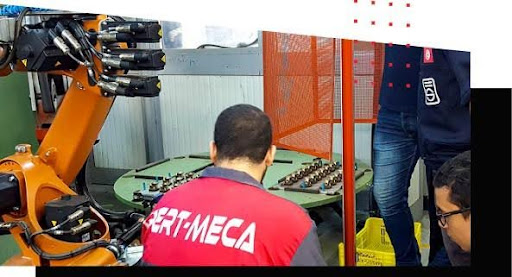
\includegraphics[width=0.6\textwidth]{Images/Chap1/AfterSales.jpg}
\caption[ After-sales service zone]{After-sales service zone}
\label{fig:XPERT-MECA_AfterSales}
\end{figure}

\subsection{Procurement Team}
This team is responsible for the strategic management of the supply chain, from sourcing materials to inventory management. They handle the procurement of all necessary components and materials for production, including electronic parts, mechanical components, and raw materials. The team carefully selects and vets suppliers to ensure that all resources meet quality standards and are available in a timely manner. Their efficient management of the supply process is critical for maintaining smooth manufacturing operations and controlling project costs. Figure \ref{fig:XPERT-MECA_Procurement} provides a look at the procurement and storage area.

\begin{figure}[H]
\centering
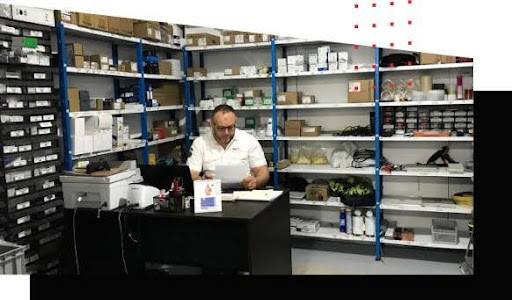
\includegraphics[width=0.6\textwidth]{Images/Chap1/Procurement.jpg}
\caption[Procurement and storage area]{ Procurement and storage area}
\label{fig:XPERT-MECA_Procurement}
\end{figure}
\section{External Ecosystem and Collaborations}
\subsection{Business Sectors}
Xpert-Meca extends its expertise in robotics and automation across a diverse range of industrial sectors, providing tailored solutions that address the specific needs of each market. The company’s strategic focus on these key industries allows for the development of highly specialized applications that enhance productivity, quality, and safety.

\begin{itemize}
\item \textbf{Agro-food Sector}: In this industry, Xpert-Meca focuses on automating processes that require precision and hygiene, such as handling, packaging, and sorting. Robotic solutions are employed to increase throughput and ensure consistency in food production lines;
\item \textbf{Automotive Sector}: This is a core area for the company, where robust robotic applications are essential. Xpert-Meca provides advanced solutions for critical tasks like robotic welding, material handling, assembly, and quality inspection, leveraging the precision of KUKA robots;
\item \textbf{General Industrial Sector}: The company offers customized automation solutions for a broad range of general manufacturing and assembly applications. This includes the design and production of special-purpose machines for specific client requirements, optimizing various stages of the manufacturing process;
\item \textbf{Educational Sector}: In collaboration with academic institutions and technical training centers, Xpert-Meca supplies educational robotic platforms and provides specialized training. This helps prepare future engineers and technicians for modern industrial environments by giving them hands-on experience with advanced robotics and automation systems.
\end{itemize}

\subsection{Clients}
Xpert-Meca’s clients include companies from various industrial domains, ranging from local manufacturers to multinational groups seeking innovative robotic and automation solutions. The logos of some of Xpert-Meca's key clients are presented in Figure \ref{fig:ClientsLogos}.

    \begin{figure}[H]
    \centering
    
\includegraphics[width=1\textwidth]{Images/Chap1/ClientsLogos.jpg}
    \caption[ Clients Logos ]{ Clients Logos }
    \label{fig:ClientsLogos}
    \end{figure}

\subsection{Partners}
The official partners of Xpert-Meca are:

\begin{itemize}
    \item \textbf{KUKA}, a global automation corporation, is a leading provider of intelligent automation solutions. Founded in Augsburg, Germany, in 1898 by Johann Josef Keller and Jakob Knappich, the company's name is an abbreviation of "Keller und Knappich Augsburg". Since its inception, KUKA has been at the forefront of technological innovation, expanding its offerings from initial products like acetylene gas lighting to a wide range of industrial applications today;
    
    KUKA provides everything from industrial robots and software to fully automated production systems and their connectivity. The company serves various markets, including automotive (with a focus on e-mobility), electronics, metal and plastic, consumer goods, e-commerce, and healthcare. As of 2024, KUKA has approximately 15,000 employees and operates in more than 50 countries with over 100 locations.
    
    
    \item \textbf{Optimal Business Growth (OBG)} is a company based in Tunisia that offers digital transformation services to businesses, particularly in the field of IT and digitalization. They focus on assisting companies in optimizing their productivity, improving their efficiency, and increasing their profitability through technology\hyperref[sec:bibliography]{[2]}.
\end{itemize}

    
\section{Project Framework}
This section provides a comprehensive overview of the project's foundation, from the initial problem to the final solution. It details the core objectives and the principles guiding the development of the automated sorting cell.
\subsection{Problem Statement}
In the context of technology fairs and industrial exhibitions, there is a clear need for demonstrations that are not only dynamic and visually appealing, but also educational. The challenge is to create an engaging showcase that effectively highlights the core principles of Industry 4.0, such as robotics and automation, in a way that is easily accessible and understandable to a broad audience. This project addresses this need by developing an inspiring, interactive demonstration that leverages modern automation principles to spark visitor interest and engagement.

\subsection{Project Objective}
The main goal of this project is to design and implement an interactive and visual demonstration system that serves as a powerful showcase for advanced industrial technologies. The system must be developed to be showcased at industrial fairs or tech events, with the following key objectives:
\begin{itemize}
\item \textbf{Showcase Robotics Capabilities:} Highlight the precision, speed, and reliability of industrial robots in a dynamic and safe environment;
\item \textbf{Illustrate System Integration:} Clearly demonstrate the seamless coordination and communication between various subsystems, including robots, vision systems, and conveyors;
\item \textbf{Engage and Educate the Audience:} Capture visitors' attention through a smooth, colorful, and highly visual demonstration, while making the underlying principles of automation easy to understand;
\item \textbf{Validate the Full Development Cycle:} Prove the project's success by executing the full engineering process, from initial design and part selection to the final implementation and automation of the solution.
\end{itemize}

\subsection{Project Solution and Operating Principle}
To address the need for a dynamic and educational demonstration, the project solution is the design and implementation of a fully automated cube handling and sorting cell. This cell serves as a sophisticated showcase of modern industrial automation and robotics principles.
\newline
The system's core is the KUKA KR AGILUS industrial robot, which performs precise pick-and-place operations. Cubes of various colors are fed into the system via two motorized belt conveyors. Their presence is detected by sensors, while a vision system powered by a Raspberry Pi and a camera identifies the color of each cube. The robot then retrieves the cubes and sorts them into their designated bins based on the color detected.

The entire process is automated and runs in a continuous loop, which makes it ideal for uninterrupted demonstrations at industrial exhibitions. The system's operation is governed by a repetitive, automated, and visual cycle:

\begin{itemize}
\item \textbf{Cube Transportation:} Cubes of different colors are transported by motorized conveyors;
\item \textbf{Presence Detection:} Their presence is detected by a series of sensors, which signal the system to begin the next phase;
\item \textbf{Color Analysis:} An industrial camera, placed strategically, analyzes the color of the cube;
\item \textbf{Robotic Sorting:} The KUKA robot picks up the cubes with a custom gripper and places them into dedicated bins based on the detected color;
\item \textbf{Cycle Restart:} Once sorted, the cubes are recirculated back onto the conveyor to restart the cycle continuously.
\end{itemize}

The entire system's logic and sequencing are managed by a Siemens PLC, while an HMI provides real-time feedback and control, ensuring the system is both functional and transparent for any audience.

\subsection{System Flowchart}
To provide a clear, high-level overview of the system's operational flow, the diagram in annex \ref{fig:Flowchart} illustrates the sorting cell's general behavior from initialization to cube classification. It simplifies the cycle into key actions and shows how the different components interact in a sequential manner.



\subsection{Added Value}
The robotic sorting cell is designed not only as a functional system but also as a strategic tool for showcasing advanced technology. Its core value proposition can be broken down into the following key benefits:

\begin{itemize}
\item \textbf{Interactivity}: The system's precise and fluid movements, combined with the visual appeal of sorting colorful objects, naturally captures and holds the attention of visitors. This dynamic behavior transforms a passive observation into an active viewing experience, making it a compelling centerpiece for any exhibition booth. This interactivity is key to generating interest and engaging potential clients and students;

\item \textbf{Educational aspect}: The demonstration provides a practical, easy-to-understand model for explaining complex principles of automation, industrial vision, and robotics. By observing the system's simple, repetitive cycle, visitors can grasp concepts such as sensor-based feedback loops, robotic path planning, and vision-based decision-making. This hands-on, visual learning experience makes advanced technology accessible to a wider audience, from engineering students to industry professionals;

\item \textbf{Flexibility and modularity}: The system's design is inherently flexible, allowing it to be easily reconfigured to fit different exhibition spaces or to adapt to specific demonstration needs. The modularity of its components—such as the conveyors, sensors, and vision system—means it can be adjusted to showcase various levels of technical complexity, from a basic sorting task to more advanced applications, without requiring a full redesign;

\item \textbf{Innovative image}: By demonstrating expertise in advanced robotics, system integration, and smart automation, the project significantly enhances Xpert-Meca's reputation as a forward-thinking, innovative company. The showcase acts as a tangible proof of concept, highlighting the company’s capabilities in designing and implementing turnkey solutions that meet the demands of Industry 4.0. This reinforces brand image and builds confidence among partners and potential clients.
\end{itemize}

\subsection{Use in Industrial Fairs}
The entire project was conceived with a clear focus on its application in industrial fairs and technology events. The interactive booth experience is designed to be a highly effective marketing and educational tool where visitors can:

\begin{itemize}
\item \textbf{Watch the system running live:} The continuous, automated cycle of the sorting cell provides a captivating live demonstration. This allows visitors to see the robot, conveyors, and sensors working in perfect harmony, showcasing the system's reliability and the speed of modern automation in real-time. This live display is far more impactful than a static presentation or video;
\item \textbf{Talk with operators to better understand how it works:} The presence of knowledgeable operators allows for direct engagement with the audience. This interaction is crucial for translating the visual demonstration into a clear understanding of the underlying principles. Operators can explain the PLC logic, the vision system's decision-making process, and the mechanical functions, answering questions and providing deeper insights tailored to each visitor's background;
\item \textbf{Potentially take part in certain steps under supervision:} By allowing visitors to participate in simple, supervised actions—such as placing a cube on the conveyor—the booth provides a memorable and personal experience. This small act of interaction breaks down the barrier between the audience and the technology, making them feel part of the process and reinforcing the system's user-friendliness and accessibility.
\end{itemize}

\subsection{Conclusion}
This first chapter gave an overview of the project and its general context by presenting the host company. It provided a solid foundation to better understand the industrial environment in which the project takes place, including the company's main activities, clients, and partners.